\documentclass{article}
%\documentclass{pnastwo}

\usepackage{amsmath, amsthm, amsfonts, amssymb}
\usepackage{graphicx,hyperref}
\usepackage{microtype, parskip}
\usepackage[comma,sort&compress]{natbib}
\usepackage{docmute}
\usepackage{subcaption, multirow, morefloats}
\usepackage{wrapfig, rotating}


\captionsetup[subfigure]{position = top, labelfont = bf, textfont = normalfont, singlelinecheck = off, justification = raggedright}

\title{Corrections to ``Expected time-invariant effects of biological traits on mammal species durations''}
\author{Peter D Smits\\Committee on Evolutionary Biology, University of Chicago}
%\author{Peter D Smits\affil{1}{Committee on Evolutionary Biology, University of Chicago, Chicago, Illinois, USA}}

\begin{document}

\maketitle

It was recently brought to the author's attention a series of errors in the body mass data recorded in Supplementary Dataset 1 of \citep{Smits2015} which were then included in that analysis. These errors took three forms: 1) improperly back-transforming body mass data from \citet{Smith2004}, 2) incorrectly inserting the measurement of the part used to estimate body mass into the body mass column for the ``PBDB + regression'' observations, and 3) improperly transforming rodent log mass estimated as a part of this study. The first error affects 24 of 1936 observations, the second affects approximately 1000 of the observations, and the third error affects an unknown set of observations.

All three of these errors were caused by errors in the code processing all of the collected body size data. The first error was due to the body mass data recorded by \citet{Smith2004} was log base 10 transformed and not natural log transformed; I made the mistake and back-transformed by raising \(e\) to that power instead of 10. The second error was also the product of a minor coding mistake. In the code for processing body mass data from all the different sources, those which are processed as ``PBDB + regression'' have an intermediate step with four columns; I used the incorrect column call which caused this error. The third error was involved with predicting rodent mass from lower first molar area. The regression formula used to estimate mass uses log of area of lower first molar and gives log mass. Instead of exponentiating that log mass to put it in grams, I accidentally log transformed the log mass value again. What this produces a number of mass estimates below 2 grams, which is unrealistic given that this is the approximate minimum for mammal body size \citep{Smith2004,Smith2011f}. 

The original analyses of \citep{Smits2015} were re-run using the updated and corrected body mass estimates. Quantitatively, the subtle aspects of the estimates have moved slightly but not substantially enough to change the original results. Qualitatively, there is no difference in the conclusions that can be made from these new results. Whatever changes to the parameter estimates which may have occurred are most observable in Table \ref{tab:new_res} which is a remake of Table 1 from \citet{Smits2015}; the mean and median of the posterior distributions for each parameter have changed by approximately 0.01. The newly made figures from this re-analysis are presented in the new Supplementary Information for this correction.

Additionally, Supplementary Dataset 1 from \citet{Smits2015} was modified with an additional column titled ``suspicious.'' those entries marked as suspicious are those deemed by Chrstine Janis to be worthy of improvement (personal communication). A comparison of the body mass distribution of the suspicious and not suspicious indicates that the suspicious body mass values are relatively evenly distributed across the entire distribution (Fig. \ref{fig:body_size}); this is also the case for the cohort-specific body size distributions (Fig. \ref{fig:body_size_time}).

An archive of the original, uncorrected code is available at http://dx.doi.org/10.5281/zenodo.44365. An archive of the new, corrected code is available at https://github.com/psmits/cosmo\_prov. The first two errors take place in file R/body\_size.r on lines 48-49 and 160-161, respectively. The third error is found in file R/predict\_mass.r on line 207. No other code changes were necessary to correct these errors.


\begin{figure}[ht]
  \centering
  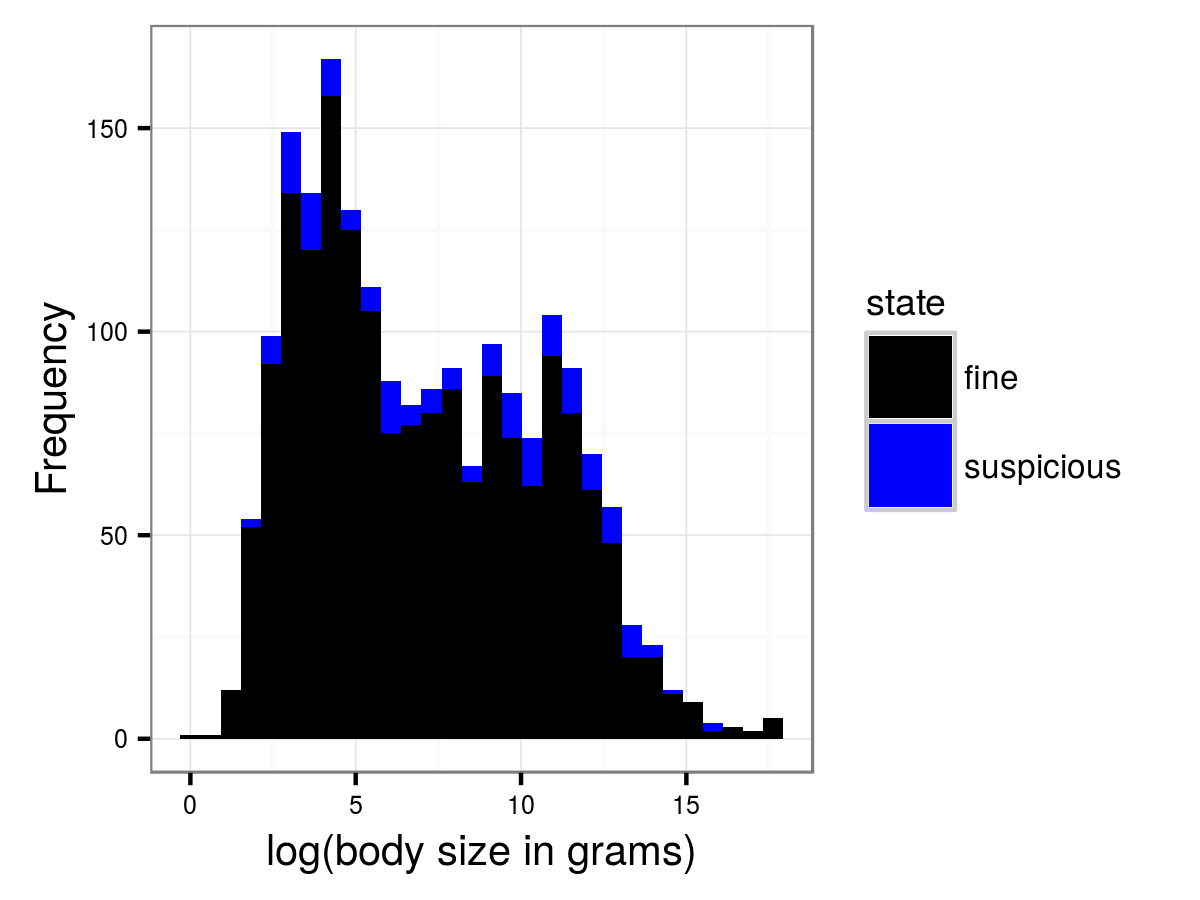
\includegraphics[height=0.4\textheight, width=\textwidth, keepaspectratio=true]{figure/body_size_compare}
  \caption{Histogram of mammal body sizes analyzed as a part of \citet{Smits2015}. Labeled in black are non-suspicious body sizes, while those labeled in blue are those observations that are still considered suspicious (Janis, personal communication).}
  \label{fig:body_size}
\end{figure}

\begin{figure}[ht]
  \centering
  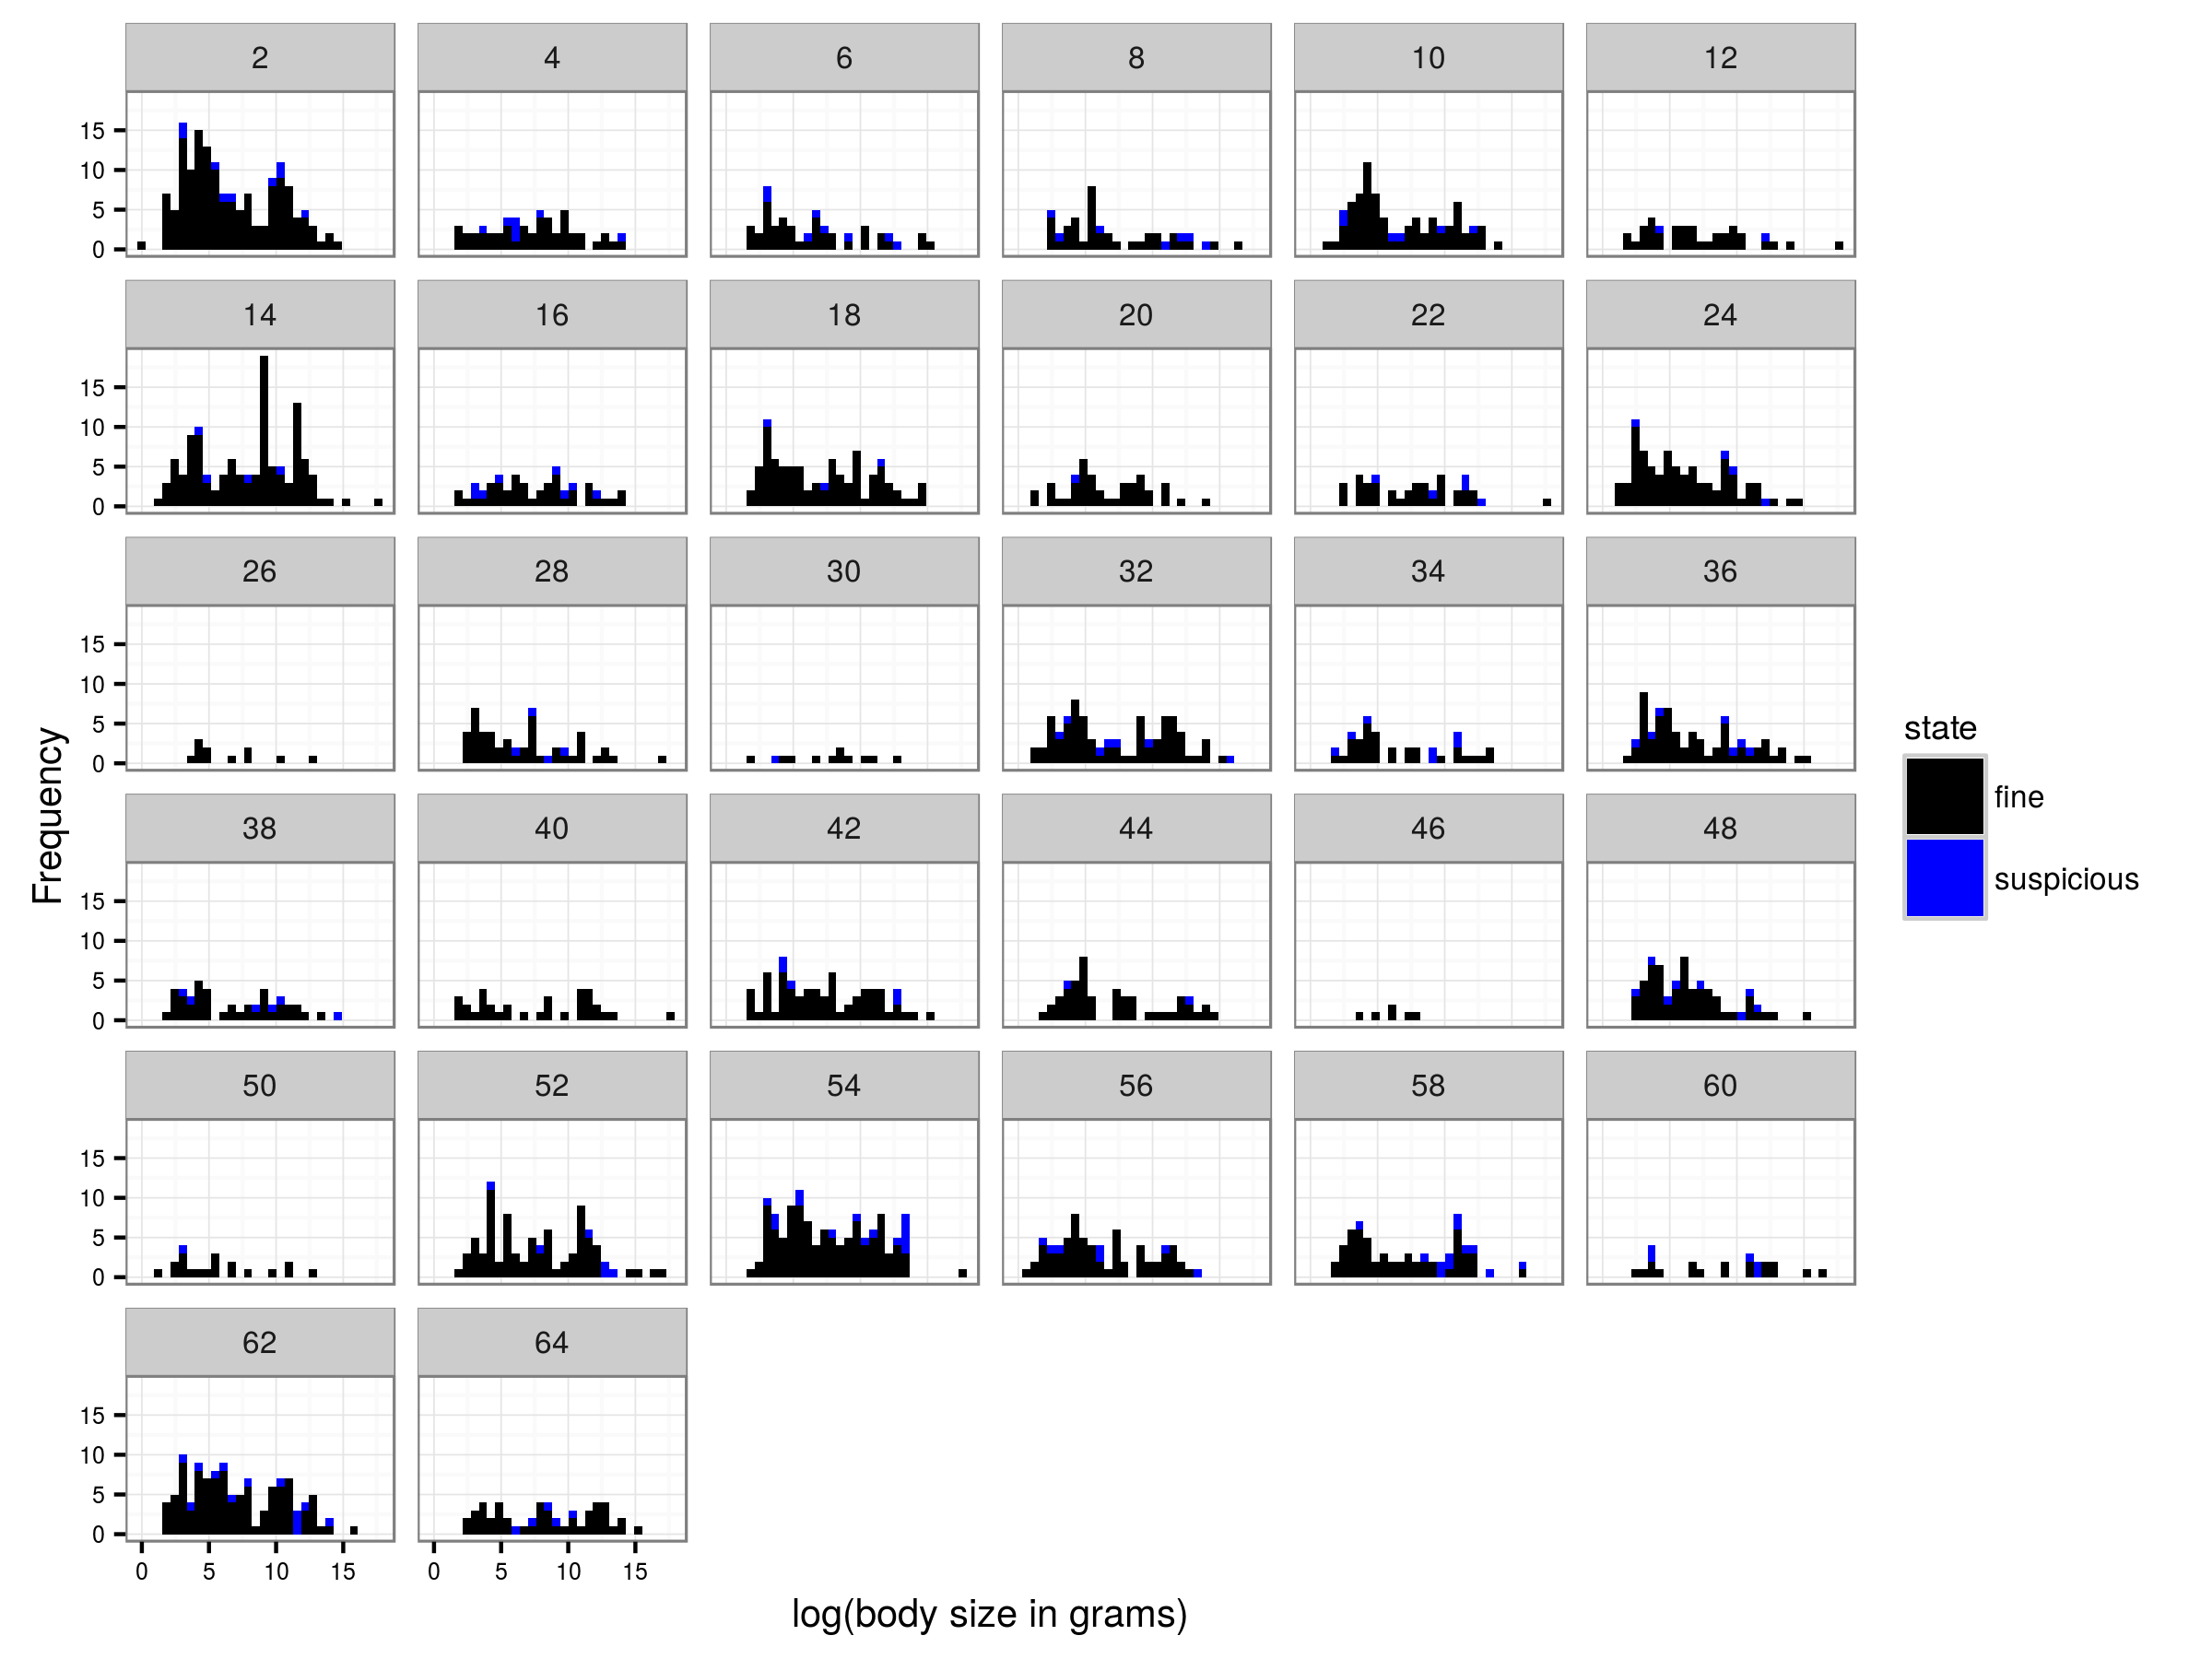
\includegraphics[height=0.6\textheight, width=\textwidth, keepaspectratio=true]{figure/body_size_compare_time}
  \caption{Histograms of mammal body sizes for each origination cohort. As in Figure \ref{fig:body_size}, body sizes are labeled as suspicious (blue) or not (black). Each origination cohort is labeled as the maximum age of origination, in millions of years, for that cohort.}
  \label{fig:body_size_time}
\end{figure}

\begin{table}[c]
  \centering
  \caption{Marginal posterior estimates for the parameters of interested based on 1000 posterior samples. The intercept \(\beta_{0}\) can also be interpreted as the estimate for the mean observed species. The remaining \(\beta\) values can be interpreted as the effect of a trait on the expected species duration as expressed as deviation from the mean. The categorical variables are binary index variables where an observation is of that category or not. See \citet{Smits2015} for explainations of the parameters and their estimates.}
  \begin{tabular}{ l l r r r r r r r r }
    parameter & effect & mean & sd & 2.5\% & 25\% & 50\% & 75\% & 97.5\% & \(\hat{R}\) \\ 
    \hline
    \(\alpha\) & ``age'' &1.29 & 0.03 & 1.23 & 1.27 & 1.29 & 1.31 & 1.36 & 1.02 \\ 
    \hline
    \(\beta_{0}\) & arboreal/carnivore & -0.78 & 0.14 & -1.06 & -0.88 & -0.78 & -0.69 & -0.50 & 1.01 \\ 
    \(\beta_{o}\) & occupancy & -0.57 & 0.08 & -0.73 & -0.63 & -0.57 & -0.52 & -0.41 & 1.00 \\ 
    \(\beta_{size}\) & body size & 0.01 & 0.05 & -0.08 & -0.02 & 0.02 & 0.05 & 0.11 & 1.00 \\ 
    \(\beta_{g}\) & ground dwelling & -0.27 & 0.09 & -0.45 & -0.33 & -0.27 & -0.21 & -0.08 & 1.00 \\ 
    \(\beta_{s}\) & scansorial & -0.21 & 0.11 & -0.43 & -0.28 & -0.21 & -0.14 & -0.01 & 1.00 \\ 
    \(\beta_{h}\) & herbivore & 0.08 & 0.09 & -0.09 & 0.02 & 0.08 & 0.14 & 0.26 & 1.00 \\ 
    \(\beta_{i}\) & insectivore & 0.08 & 0.11 & -0.13 & 0.01 & 0.08 & 0.15 & 0.29 & 1.00 \\ 
    \(\beta_{o}\) & omnivore & -0.13 & 0.10 & -0.34 & -0.20 & -0.13 & -0.06 & 0.07 & 1.00 \\ 
    \hline
    \(\sigma_{c}\) & sd cohort & 0.34 & 0.07 & 0.24 & 0.30 & 0.33 & 0.38 & 0.50 & 1.00 \\ 
    \(\sigma_{p}\) & sd phylogeny & 0.11 & 0.06 & 0.02 & 0.07 & 0.10 & 0.15 & 0.25 & 1.07 \\ 
    \hline
  \end{tabular}
  \label{tab:new_res}
\end{table}



\pagebreak 

\bibliographystyle{abbrvnat}
%\bibliographystyle{pnas}
\bibliography{biblio}

\end{document}
